% =============================================================================
%  portopt : methodology (English version)
%  Build: cd docs && latexmk -xelatex methodology_en.tex
% =============================================================================
\documentclass[11pt,a4paper]{article}

% ----------------------------------------------------------------- language, fonts
\usepackage{polyglossia}
\setdefaultlanguage[variant=american]{english}
\usepackage{amsmath,amssymb,amsthm,mathtools}
\usepackage[math-style=ISO,bold-style=ISO]{unicode-math}
\setmainfont{Latin Modern Roman}[SmallCapsFont={Latin Modern Roman Caps}]
\setmathfont{Latin Modern Math}
\setsansfont{space-grotesk-400.ttf}[
  Path=../portopt/fonts/, BoldFont=space-grotesk-600.ttf, Scale=0.95,
  SmallCapsFont=space-grotesk-400.ttf, BoldFeatures={SmallCapsFont=space-grotesk-600.ttf}]
\setmonofont{space-mono-400.ttf}[Path=../portopt/fonts/, Scale=0.86]
\newfontfamily\headfont{space-grotesk-600.ttf}[Path=../portopt/fonts/]
\usepackage[autostyle]{csquotes}

% ----------------------------------------------------------------- layout
\usepackage[a4paper,margin=2.5cm,headheight=14pt]{geometry}
\usepackage{microtype}
\usepackage{xcolor}
\definecolor{accent}{HTML}{2A78D6}
\definecolor{accentsoft}{HTML}{F2F7FD}
\definecolor{warm}{HTML}{EB6834}
\definecolor{warmsoft}{HTML}{FDF3EE}
\definecolor{green}{HTML}{1BAF7A}
\definecolor{greensoft}{HTML}{EEFAF5}
\definecolor{ink}{HTML}{0B0B0B}
\definecolor{ink2}{HTML}{52514E}
\definecolor{rule}{HTML}{E4E3DF}

\usepackage{graphicx}
\graphicspath{{figures/}}
\usepackage[font=small,labelfont={sf,bf},labelsep=period,skip=6pt]{caption}
\usepackage{booktabs,tabularx,array}
\usepackage[section]{placeins}
\usepackage{enumitem}
\setlist{itemsep=2pt,topsep=4pt,leftmargin=*}
\usepackage{fancyhdr}
\usepackage{titlesec}
\usepackage[most]{tcolorbox}
\usepackage{listings}
\usepackage{tikz}
\usetikzlibrary{positioning,arrows.meta}
\usepackage[ruled,vlined,linesnumbered]{algorithm2e}
\usepackage[round,authoryear]{natbib}
\usepackage[hidelinks]{hyperref}
\hypersetup{colorlinks=true,linkcolor=accent,citecolor=accent,urlcolor=accent,
  pdftitle={portopt: methodology},
  pdfauthor={Jean Philippe N'DRI}}

% ----------------------------------------------------------------- headings
\titleformat{\section}{\headfont\Large\color{ink}}{\color{accent}\thesection}{0.8em}{}
\titleformat{\subsection}{\headfont\large\color{ink}}{\color{accent}\thesubsection}{0.7em}{}
\titleformat{\subsubsection}{\headfont\normalsize\color{ink}}{}{0em}{}
\titlespacing*{\section}{0pt}{2.2ex plus .5ex}{1.2ex}
\titlespacing*{\subsection}{0pt}{1.8ex plus .4ex}{0.9ex}
\titlespacing*{\subsubsection}{0pt}{1.4ex plus .3ex}{0.5ex}
\setcounter{secnumdepth}{2}
\setcounter{tocdepth}{2}

\pagestyle{fancy}
\fancyhf{}
\renewcommand{\headrulewidth}{0.4pt}
\renewcommand{\headrule}{\color{rule}\hrule height\headrulewidth}
\fancyhead[L]{\sffamily\footnotesize\color{ink2}portopt \textperiodcentered{} Documentation}
\fancyhead[R]{\sffamily\footnotesize\color{ink2}\nouppercase{\leftmark}}
\fancyfoot[C]{\sffamily\footnotesize\color{ink2}\thepage}
\renewcommand{\sectionmark}[1]{\markboth{\thesection\quad #1}{}}

% ----------------------------------------------------------------- statements
\newtheoremstyle{pstate}{8pt}{8pt}{\itshape}{}{\sffamily\bfseries\color{ink}}{.}{0.5em}{}
\newtheoremstyle{pdef}{8pt}{8pt}{}{}{\sffamily\bfseries\color{ink}}{.}{0.5em}{}
\theoremstyle{pdef}
\newtheorem{definition}{Definition}[section]
\theoremstyle{pstate}
\newtheorem{proposition}[definition]{Proposition}
\newtheorem{theorem}[definition]{Theorem}
\newtheorem{lemma}[definition]{Lemma}
\renewcommand{\qedsymbol}{\ensuremath{\blacksquare}}
\makeatletter
\renewenvironment{proof}[1][\proofname]{\par\pushQED{\qed}\normalfont
  \topsep6pt\trivlist\item[\hskip\labelsep{\sffamily\bfseries #1.}]\ignorespaces}
  {\popQED\endtrivlist\@endpefalse}
\makeatother
\newcommand{\admitted}[1]{{\upshape\small\color{ink2}(admitted, #1)}}

% ----------------------------------------------------------------- boxes
\tcbset{pbox/.style={enhanced,breakable,boxrule=0pt,arc=2pt,outer arc=2pt,
  left=10pt,right=10pt,top=6pt,bottom=6pt,before skip=10pt,after skip=10pt,
  fonttitle=\sffamily\bfseries\small,coltitle=ink,
  attach title to upper={\par\smallskip},fontupper=\small\raggedright}}
\newtcolorbox{code}{pbox,colback=accentsoft,borderline west={2.5pt}{0pt}{accent},title={In the code}}
\newtcolorbox{practice}{pbox,colback=warmsoft,borderline west={2.5pt}{0pt}{warm},title={In practice}}
\newtcolorbox{example}[1][Example]{pbox,colback=greensoft,borderline west={2.5pt}{0pt}{green},title={#1}}

\lstset{basicstyle=\ttfamily\small,columns=fullflexible,keepspaces=true,
  backgroundcolor=\color{accentsoft},frame=none,xleftmargin=8pt,xrightmargin=8pt,
  aboveskip=8pt,belowskip=8pt,commentstyle=\color{ink2},keywordstyle=\color{accent},
  stringstyle=\color{warm},language=Python,showstringspaces=false,upquote=true}

% ----------------------------------------------------------------- algorithms
\SetAlFnt{\small}
\SetAlCapFnt{\sffamily\bfseries\small}
\SetAlCapNameFnt{\small}
\SetKwComment{Com}{\color{ink2}\# }{}
\SetArgSty{textnormal}
\SetKw{KwRet}{return}

% ----------------------------------------------------------------- macros
\newcommand{\py}[1]{{\ttfamily\hyphenchar\font=-1 \detokenize{#1}}}
\newcommand{\R}{\mathbb{R}}
\newcommand{\E}{\mathbb{E}}
\newcommand{\one}{\mathbf{1}}
\newcommand{\T}{^{\top}}
\newcommand{\pct}{\%}
\newcommand{\simplex}{\Delta_N}
\DeclareMathOperator{\tr}{tr}
\DeclareMathOperator{\Cov}{Cov}
\DeclareMathOperator{\Var}{Var}
\DeclareMathOperator{\diag}{diag}
\DeclareMathOperator{\se}{se}
\newcommand{\SR}{\mathrm{SR}}
\newcommand{\SRh}{\widehat{\mathrm{SR}}}
\newcommand{\VaR}{\mathrm{VaR}}
\newcommand{\CVaR}{\mathrm{CVaR}}
\newcommand{\CAGR}{\mathrm{CAGR}}
\newcommand{\MaxDD}{\mathrm{MaxDD}}
\newcommand{\RC}{\mathrm{RC}}
\newcommand{\MRC}{\mathrm{MRC}}
\newcommand{\sMV}{\sigma_{\mathrm{MV}}}
\newcommand{\sERC}{\sigma_{\mathrm{ERC}}}
\newcommand{\sEW}{\sigma_{1/N}}
\newcommand{\fig}[3][\linewidth]{%
  \begin{figure}[htbp]\centering\includegraphics[width=#1]{#2}\caption{#3}\label{fig:#2}\end{figure}}

\setlength{\parindent}{0pt}
\setlength{\parskip}{5pt plus 1pt}
\setlength{\emergencystretch}{2em}
\renewcommand{\arraystretch}{1.15}

% =============================================================================
\begin{document}

% ----------------------------------------------------------------- title
\begin{titlepage}
\newgeometry{margin=2.5cm,top=3cm}
{\sffamily\small\color{ink2}portopt \textperiodcentered{} Documentation \textperiodcentered{} v0.1.0}

\vspace{3.2cm}
{\headfont\fontsize{30}{36}\selectfont\color{ink} Risk-based\\[4pt] portfolio allocation\par}
\vspace{10pt}
{\color{accent}\rule{3.2cm}{2.5pt}}
\vspace{14pt}

{\sffamily\Large\color{ink2} A guide to the portopt library:\\ definitions, results and proofs\par}

\vspace{1.4cm}
\begin{minipage}{0.86\linewidth}\small
\py{portopt} compares risk-based allocation rules (1/N, inverse volatility, risk
budgeting, ERC, HRP) in a walk-forward backtest, then measures their performance and
risk. This guide first introduces the library, then covers each building block with the
same structure: definition, result, proof, call in the code. Every stated result is
either proved or flagged as admitted, with its reference.
\end{minipage}

\vfill
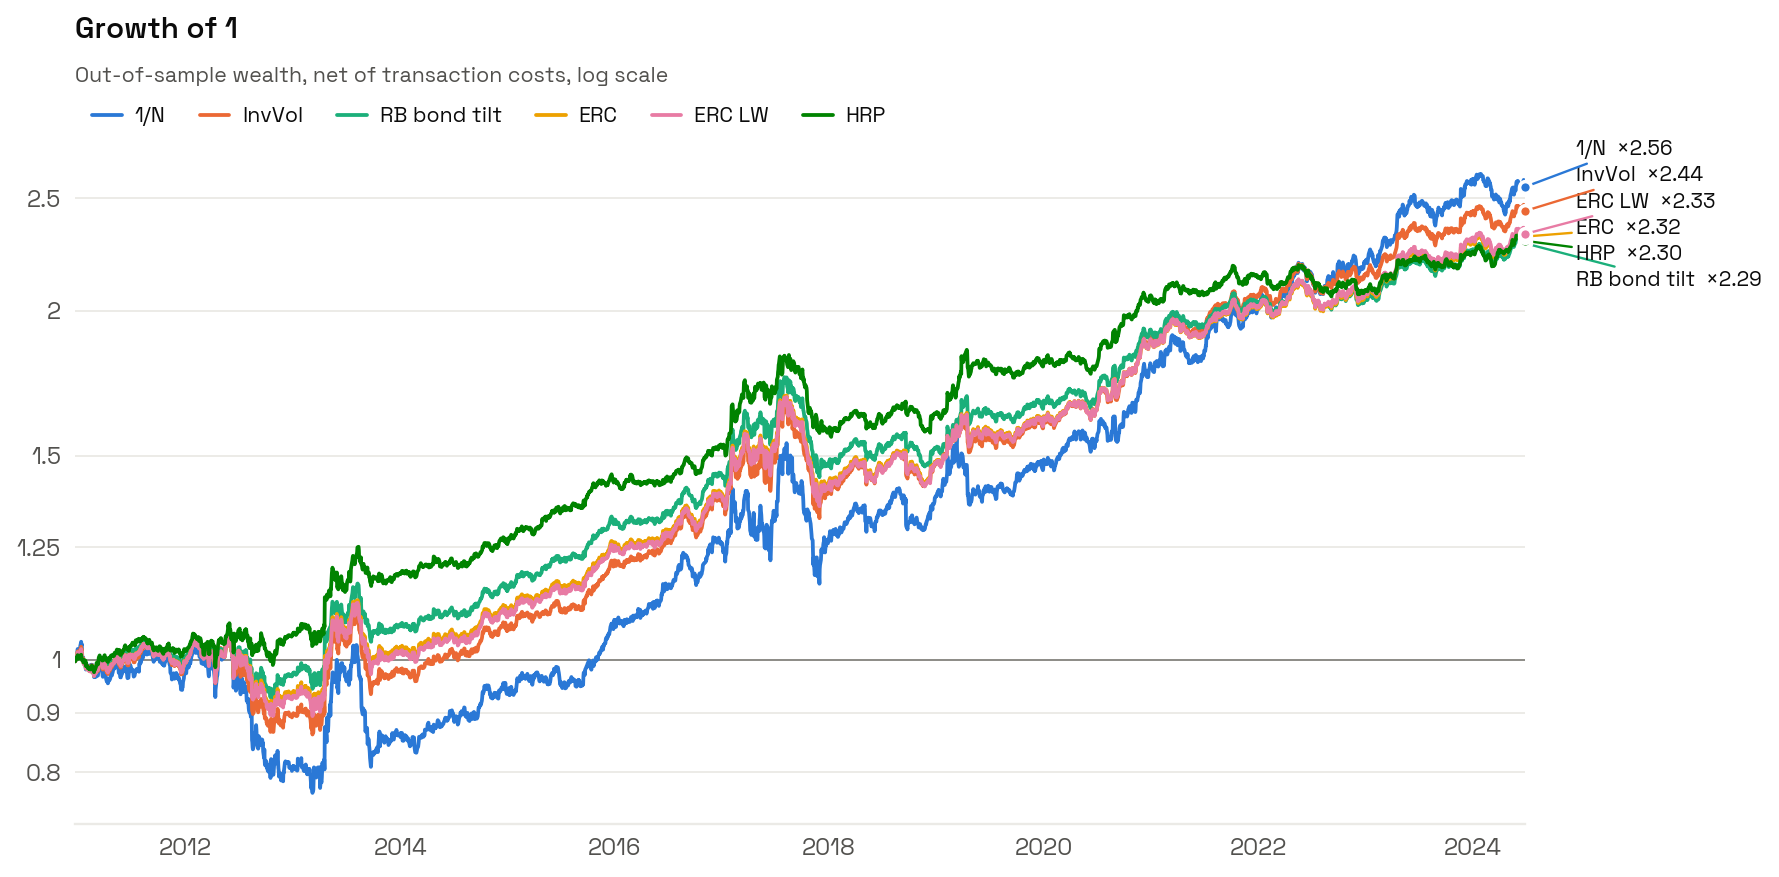
\includegraphics[width=\linewidth]{report_01_wealth.png}

\vspace{1cm}
{\sffamily\small
\begin{tabular}{@{}l@{\hspace{1.2cm}}l@{}}
\color{ink2}Author & Jean Philippe N'DRI \\
\color{ink2}Version & September 2026 \\
\color{ink2}Code & \py{portopt/}
\end{tabular}}
\restoregeometry
\end{titlepage}

{\hypersetup{linkcolor=ink}\tableofcontents}
\thispagestyle{fancy}
\newpage

% =============================================================================
\section{Getting started}\label{sec:start}

\subsection{What the library does}

\py{portopt} answers one question: \emph{which allocation rule would have delivered the
best return/risk trade-off, without using any future information?} It follows a
four-step flow, one module per step.

\begin{center}
\begin{tikzpicture}[
  box/.style={draw=accent,fill=accentsoft,rounded corners=3pt,line width=0.8pt,
    minimum width=2.75cm,minimum height=1.3cm,align=center,font=\sffamily\small},
  lab/.style={font=\scriptsize,text=ink2,align=center},
  arr/.style={-{Stealth[length=6pt]},line width=0.8pt,color=ink2}]
\node[box] (d) {\textbf{data}\\[1pt]{\scriptsize prices $\to$ returns}};
\node[box,right=1.15cm of d] (e) {\textbf{estimator}\\[1pt]{\scriptsize window $\to$ weights}};
\node[box,right=1.15cm of e] (b) {\textbf{backtester}\\[1pt]{\scriptsize weights $\to$ returns}};
\node[box,right=1.15cm of b] (m) {\textbf{metric, plot}\\[1pt]{\scriptsize returns $\to$ report}};
\draw[arr] (d) -- node[above,lab]{$R$} node[below,lab]{$T\times N$} (e);
\draw[arr] (e) -- node[above,lab]{$w$} node[below,lab]{$N$} (b);
\draw[arr] (b) -- node[above,lab]{$R_p$} node[below,lab]{$T-L$} (m);
\end{tikzpicture}
\end{center}

\begin{enumerate}
\item \textbf{data} downloads prices, cleans them and computes the returns $R$, a
\py{DataFrame} of $T$ dates by $N$ assets (section~\ref{sec:data}).
\item \textbf{estimator} turns a window of returns into weights $w$: this is the
\emph{allocation rule} (sections~\ref{sec:cov} to~\ref{sec:alloc}).
\item \textbf{backtester} applies the rule at every rebalancing date, lets the portfolio
evolve between dates and returns its out-of-sample returns $R_p$
(section~\ref{sec:backtest}).
\item \textbf{metric} and \textbf{plot} summarize these returns into metrics and charts
(sections~\ref{sec:perf} to~\ref{sec:stats}).
\end{enumerate}

\subsection{First backtest}

\begin{lstlisting}
pip install -e ".[dev]"      # numpy, pandas, scipy, yfinance, matplotlib, pytest
\end{lstlisting}

\begin{lstlisting}
from portopt import load_returns, EqualWeight, ERC, HRP, run_backtests, summary
from portopt import plot

# 1. data: daily returns, T dates x N assets
R = load_returns(["SPY", "TLT", "GLD", "DBC", "EFA"], start="2008-01-01")

# 2. estimator: the allocation rules to compare
rules = {"1/N": EqualWeight(), "ERC": ERC(), "HRP": HRP()}

# 3. backtester: 252-day window, rebalancing every 21 days
rets, bts = run_backtests(R, rules, in_sample=252, out_of_sample=21,
                          transaction_cost_bps=5)

# 4. metric and plot
print(summary(rets))
plot.save_report(rets, bts, "outputs/charts")
\end{lstlisting}

\py{rets} holds one daily out-of-sample return per strategy, and
\py{bts["ERC"].weights_} the ERC weights at each rebalancing. Without network access,
the \py{simulate_returns()} function of the \py{data} module provides a simulated
universe of 10 ETFs.

\subsection{Writing your own rule}

A rule inherits from \py{BaseEstimator} and implements \py{_compute_weights}. The
backtester accepts it as is.

\begin{lstlisting}
import numpy as np
from portopt import BaseEstimator

class InverseVariance(BaseEstimator):
    def _compute_weights(self, returns):
        cov = self._cov(returns)          # applies cov_method
        return 1.0 / np.diag(cov)
\end{lstlisting}

\py{fit} does the rest: it rejects windows with missing values, sets negative weights
to zero, normalizes the sum to 1 and stores the result in \py{weights_}, a
\py{pd.Series} indexed by asset.

\subsection{API map}

\begin{center}\small
\begin{tabularx}{\linewidth}{@{}l>{\raggedright}X>{\raggedright\arraybackslash}p{1.5cm}@{}}
\toprule
Object & Role & Section \\
\midrule
\py{load_returns}, \py{download_prices} & get prices and returns & \ref{sec:data} \\
\py{clean_prices}, \py{compute_returns} & clean data, compute returns & \ref{sec:data} \\
\py{simulate_returns} & simulated universe for offline work & \ref{sec:data} \\
\py{estimate_cov}, \py{ledoit_wolf_cov}, \py{ewma_cov} & estimate the covariance & \ref{sec:cov} \\
\py{risk_contributions} & risk contributions & \ref{sec:rc} \\
\py{EqualWeight}, \py{InverseVolatility} & rules without optimization & \ref{sec:ew}, \ref{sec:iv} \\
\py{RiskParity}, \py{ERC} & risk budgeting, equal contributions & \ref{sec:rb}, \ref{sec:erc} \\
\py{HRP} & Hierarchical Risk Parity & \ref{sec:hrp} \\
\py{Backtester}, \py{run_backtests} & walk-forward backtest & \ref{sec:backtest} \\
\py{summary}, \py{metric} module & performance and risk metrics & \ref{sec:perf}--\ref{sec:stats} \\
\py{plot.save_report} & chart report (PNG) & \ref{sec:example} \\
\bottomrule
\end{tabularx}
\end{center}

\subsection{Notation}

\begin{center}\small
\begin{tabularx}{\linewidth}{@{}>{$}l<{$}X@{}}
\toprule
N,\ T & number of assets, number of dates \\
R_t\in\R^N & simple returns of the assets, from the close of $t-1$ to the close of $t$ \\
\simplex & $\{w\in\R^N : w\ge0,\ \one\T w=1\}$, the set of long-only portfolios \\
\Sigma,\ \sigma_i,\ \rho_{ij} & covariance, volatilities $\sigma_i=\sqrt{\Sigma_{ii}}$, correlations \\
P & number of periods per year (252 for daily data) \\
L,\ H & estimation window length, holding period \\
\bar R,\ \hat\sigma & sample mean and standard deviation \\
\Phi,\ \varphi & cumulative distribution function and density of the standard normal \\
\bottomrule
\end{tabularx}
\end{center}

% =============================================================================
\section{Returns and portfolio}\label{sec:data}

\begin{definition}[returns]
For a price $P_t$ adjusted for dividends and splits, the simple return and the log
return are
\[
R_t=\frac{P_t}{P_{t-1}}-1,\qquad r_t=\ln\frac{P_t}{P_{t-1}}=\ln(1+R_t).
\]
\end{definition}

\begin{definition}[portfolio]
A portfolio is a vector $w\in\simplex$: $w_i$ is the share of value invested in asset
$i$. Its return is denoted $R_{p,t}$.
\end{definition}

\begin{proposition}\label{prop:simple}
If $w$ are the weights at $t-1$, then $R_{p,t}=w\T R_t$. The analogous identity is false
for log returns.
\end{proposition}

\begin{proof}
Let $n_i$ be the number of units of asset $i$ held and $V_t=\sum_in_iP_{i,t}$. Then
$V_t/V_{t-1}=\sum_i\frac{n_iP_{i,t-1}}{V_{t-1}}\cdot\frac{P_{i,t}}{P_{i,t-1}}=\sum_iw_i(1+R_{i,t})$,
hence $R_{p,t}=w\T R_t$. For log returns, $r_{p,t}=\ln\sum_iw_ie^{r_{i,t}}$, which is
strictly greater than $\sum_iw_ir_{i,t}$ as soon as the $r_{i,t}$ differ (strict
concavity of the logarithm).
\end{proof}

The whole library therefore works with \textbf{simple returns}.

\begin{definition}[portfolio volatility]
If $\Sigma$ is the covariance of returns, the variance and volatility of portfolio $w$
are $\sigma_p^2(w)=w\T\Sigma w$ and $\sigma_p(w)=\sqrt{w\T\Sigma w}$.
\end{definition}

\begin{definition}[annualization]
For returns with $P$ periods per year: $\mu_{\mathrm{ann}}=P\,\bar R$ and
$\sigma_{\mathrm{ann}}=\sqrt P\,\hat\sigma$.
\end{definition}

\begin{proposition}\label{prop:annual}
If the returns of the $P$ periods of a year are independent, with mean $\mu$ and variance
$\sigma^2$, and the annual return is their sum, then it has mean $P\mu$ and standard
deviation $\sqrt P\,\sigma$.
\end{proposition}

\begin{proof}
Expectation is linear, and by independence the variance of a sum is the sum of the
variances: $\Var\bigl(\sum_{k=1}^PX_k\bigr)=P\sigma^2$.
\end{proof}

Additivity is exact for log returns and holds to first order for daily simple returns.
This is what justifies the factors $P$ and $\sqrt P$.

\begin{code}
\py{load_returns(tickers, start, end, cache_dir="data_cache")} downloads adjusted
prices, cleans them and returns simple returns. Cleaning (\py{clean_prices}) fills gaps
of at most 5 days with the last known value, never fills with a future value, and keeps
the missing values of an asset not yet listed: the backtester only invests in it once
its history is complete.
\end{code}

% =============================================================================
\section{Estimating the covariance}\label{sec:cov}

Every rule except 1/N uses an estimate of $\Sigma$ over the window.

\begin{definition}[sample covariance]
Over a window of $T$ dates, with $x_t=R_t-\bar R$: $S=\frac{1}{T-1}\sum_{t=1}^Tx_tx_t\T$.
\end{definition}

$S$ is unbiased but noisy. It has $N(N+1)/2$ parameters and, if $T\le N$, it has rank at
most $T-1$, so it cannot be inverted.

\begin{theorem}[Marchenko-Pastur]\label{thm:mp}
If the $R_t$ are independent with covariance $I_N$ and $N,T\to\infty$ with
$N/T\to q\in(0,1]$, the eigenvalues of $S$ spread over
$\bigl[(1-\sqrt q)^2,(1+\sqrt q)^2\bigr]$. \admitted{\citealp{marchenko1967}}
\end{theorem}

Even when all true eigenvalues equal 1, those of $S$ spread from $0.09$ to $2.91$ for
$q=0.5$. Small eigenvalues are underestimated, and they are precisely the ones that
inverting $\Sigma$ amplifies.

\begin{definition}[Ledoit-Wolf]
Let $S_T=\frac1T\sum_tx_tx_t\T$, $\lVert A\rVert^2=\tr(AA\T)/N$ and $\mu=\tr(S_T)/N$.
Define
\[
d^2=\lVert S_T-\mu I\rVert^2,\quad
\bar b^2=\frac1{T^2}\sum_{t=1}^T\lVert x_tx_t\T-S_T\rVert^2,\quad
\delta^\ast=\frac{\min(\bar b^2,d^2)}{d^2}\in[0,1],\quad
\hat\Sigma=\delta^\ast\mu I+(1-\delta^\ast)S_T .
\]
\end{definition}

$d^2$ measures the distance from $S_T$ to the target $\mu I$, $\bar b^2$ the estimation
noise of $S_T$; $\delta^\ast$ is the share of the distance attributed to noise. This
choice asymptotically minimizes the quadratic error among combinations of $S_T$ and
$\mu I$ \admitted{\citealp{ledoitwolf2004}}.

\begin{proposition}\label{prop:lw}
Let $\lambda_1\ge\dots\ge\lambda_N$ be the eigenvalues of $S_T$ and $\delta^\ast>0$.
\begin{enumerate}[label=(\roman*)]
\item $\hat\Sigma$ has the same eigenvectors as $S_T$, with eigenvalues
$\delta^\ast\mu+(1-\delta^\ast)\lambda_j$, and it is positive definite.
\item Its condition number $\lambda_{\max}/\lambda_{\min}$ is lower than that of $S_T$.
\end{enumerate}
\end{proposition}

\begin{proof}
(i) If $S_Tv=\lambda v$, then $\hat\Sigma v=(\delta^\ast\mu+(1-\delta^\ast)\lambda)v$, and
these values are at least $\delta^\ast\mu>0$.
(ii) With $a=\delta^\ast\mu>0$ and $c=1-\delta^\ast$, the inequality
$\frac{a+c\lambda_1}{a+c\lambda_N}\le\frac{\lambda_1}{\lambda_N}$ is equivalent to
$a\lambda_N\le a\lambda_1$, which holds.
\end{proof}

\begin{lemma}[computing $\bar b^2$ without forming the $x_tx_t\T$]
$\sum_t\lVert x_tx_t\T-S_T\rVert_F^2=\sum_t(x_t\T x_t)^2-T\lVert S_T\rVert_F^2$.
\end{lemma}

\begin{proof}
$\lVert x_tx_t\T-S_T\rVert_F^2=(x_t\T x_t)^2-2x_t\T S_Tx_t+\lVert S_T\rVert_F^2$, and
$\sum_tx_t\T S_Tx_t=\tr\bigl(S_T\sum_tx_tx_t\T\bigr)=T\lVert S_T\rVert_F^2$.
\end{proof}

\fig[0.92\linewidth]{lw_spectrum.png}{Eigenvalues of the true covariance, the sample
covariance and Ledoit-Wolf (50 assets, 75 dates). Shrinkage lifts the small eigenvalues
and divides the condition number by 5.}

\begin{definition}[EWMA]
For a half-life $h$, let $\lambda=2^{-1/h}$ and $\omega_s=\lambda^s/\sum_u\lambda^u$,
where $s=0$ is the most recent date. Then
$\hat\Sigma=\sum_s\omega_s(R_{t-s}-\bar R_\omega)(R_{t-s}-\bar R_\omega)\T$, with
$\bar R_\omega=\sum_s\omega_sR_{t-s}$.
\end{definition}

\begin{proposition}
Over an infinite history, the effective number of observations
$(\sum_s\omega_s)^2/\sum_s\omega_s^2$ equals $(1+\lambda)/(1-\lambda)$, about 182 for
$h=63$.
\end{proposition}

\begin{proof}
$\sum_s\lambda^s=\frac1{1-\lambda}$ and $\sum_s\lambda^{2s}=\frac1{1-\lambda^2}$, so the
ratio is $\frac{1-\lambda^2}{(1-\lambda)^2}=\frac{1+\lambda}{1-\lambda}$.
\end{proof}

\begin{code}
Every rule accepts \py{cov_method="sample" | "ledoit_wolf" | "ewma"} or a function
\py{returns -> ndarray}. Directly: \py{estimate_cov(R, "ledoit_wolf")},
\py{ledoit_wolf_cov(R)} which returns \py{(Sigma, delta)}, \py{ewma_cov(R, halflife=63)}.
\end{code}

\begin{practice}
No rule in the library uses expected returns. The standard error of an annualized mean
is $\sigma/\sqrt Y$ over $Y$ years, whatever the frequency ($\pm5\pct$ for
$\sigma=16\pct$ and 10 years), whereas the error on a variance shrinks with the number
of observations: covariances are estimated much better than means.
\end{practice}

% =============================================================================
\section{Risk contributions}\label{sec:rc}

\begin{proposition}[Euler decomposition]\label{prop:euler}
For any $w$ with $\sigma_p(w)>0$:
$\dfrac{\partial\sigma_p}{\partial w}=\dfrac{\Sigma w}{\sigma_p}$ and
$\sigma_p(w)=\sum_{i=1}^Nw_i\,\dfrac{\partial\sigma_p}{\partial w_i}(w)$.
\end{proposition}

\begin{proof}
The gradient follows from differentiating $\sqrt{w\T\Sigma w}$. Then
$\sum_iw_i(\Sigma w)_i/\sigma_p=w\T\Sigma w/\sigma_p=\sigma_p$.
\end{proof}

\begin{definition}[risk contributions]
Marginal, total and relative risk contribution of asset $i$:
\[
\MRC_i=\frac{(\Sigma w)_i}{\sigma_p},\qquad\RC_i=w_i\MRC_i,\qquad
\frac{\RC_i}{\sigma_p}=\frac{w_i(\Sigma w)_i}{w\T\Sigma w}.
\]
By proposition~\ref{prop:euler}, the $\RC_i$ sum to $\sigma_p$ and the relative
contributions sum to 1.
\end{definition}

\begin{proposition}\label{prop:beta}
$\MRC_i=\beta_{i,p}\,\sigma_p=\rho_{i,p}\,\sigma_i$, where $\beta_{i,p}$ and $\rho_{i,p}$
are the beta and the correlation of asset $i$ with the portfolio.
\end{proposition}

\begin{proof}
$(\Sigma w)_i=\Cov(R_i,w\T R)=\Cov(R_i,R_p)$. With
$\beta_{i,p}=\Cov(R_i,R_p)/\sigma_p^2$ and $\rho_{i,p}=\Cov(R_i,R_p)/(\sigma_i\sigma_p)$,
both identities follow.
\end{proof}

An asset weighs on risk through its beta to the portfolio, not through its own
volatility. If it is negatively correlated with the portfolio, its contribution is
negative.

\begin{example}
60/40 equity/bond portfolio, $\sigma_E=16\pct$, $\sigma_B=6\pct$, $\rho=-0.2$:
$\sigma_p^2=0.36\cdot0.0256+0.16\cdot0.0036-0.48\cdot0.2\cdot0.0096=0.00887$, so
$\sigma_p=9.4\pct$. Then $(\Sigma w)_E=0.6\cdot0.0256-0.4\cdot0.00192=0.01459$ and
$\RC_E/\sigma_p=0.6\cdot0.01459/0.00887=98.7\pct$: a 60/40 portfolio in capital is a
99/1 portfolio in risk.
\end{example}

\begin{code}
\py{risk_contributions(w, cov)} returns the relative contributions;
\py{Backtester.risk_contributions()} gives them at every rebalancing.
\end{code}

% =============================================================================
\section{Allocation rules}\label{sec:alloc}

\begin{definition}[allocation rule]
An allocation rule is a function $\mathcal A$ that maps a window of returns
$(R_{t-L},\dots,R_{t-1})$ to a portfolio $w\in\simplex$. In the library, it is a
\py{BaseEstimator}: \py{est.fit(window).weights_}.
\end{definition}

% -----------------------------------------------------------------------------
\subsection{Equal Weight (1/N)}\label{sec:ew}

\begin{definition}
$w_i=1/N$ for all $i$.
\end{definition}

\begin{proposition}\label{prop:ew}
If all assets have volatility $\sigma$ and pairwise correlations $\rho$, then
$\sigma_{1/N}^2=\frac{\sigma^2}{N}\bigl(1+(N-1)\rho\bigr)\to\rho\sigma^2$ as $N\to\infty$.
\end{proposition}

\begin{proof}
$w\T\Sigma w=\frac1{N^2}\bigl(N\sigma^2+N(N-1)\rho\sigma^2\bigr)$.
\end{proof}

Diversification removes the risk specific to each asset but not the common risk
$\rho\sigma^2$. 1/N estimates nothing and so makes no estimation error: it is the
reference benchmark, which none of the 14 optimization models tested by
\citet{demiguel2009} significantly beats out of sample.

\begin{code}
\py{EqualWeight()}
\end{code}

% -----------------------------------------------------------------------------
\subsection{Inverse volatility}\label{sec:iv}

\begin{definition}
$w_i=\sigma_i^{-k}/\sum_j\sigma_j^{-k}$, with $k=1$ (inverse volatility) or $k=2$
(inverse variance).
\end{definition}

\begin{proposition}\label{prop:invvol}
\begin{enumerate}[label=(\roman*)]
\item If all correlations are equal, inverse volatility equalizes risk contributions:
it is the ERC portfolio (section~\ref{sec:erc}).
\item If $\Sigma$ is diagonal, inverse variance is the minimum variance portfolio.
\end{enumerate}
\end{proposition}

\begin{proof}
(i) With $w_i=c/\sigma_i$ and $\rho_{ij}=\rho$ for $i\ne j$:
$(\Sigma w)_i=\sum_j\rho_{ij}\sigma_i\sigma_j\,c/\sigma_j=c\,\sigma_i\bigl(1+(N-1)\rho\bigr)$,
so $w_i(\Sigma w)_i=c^2\bigl(1+(N-1)\rho\bigr)$ does not depend on $i$.
(ii) The minimum variance portfolio is $w\propto\Sigma^{-1}\one$ and, for a diagonal
$\Sigma$, $\Sigma^{-1}\one=(\sigma_i^{-2})_i$.
\end{proof}

\begin{code}
\py{InverseVolatility(exponent=1)}; \py{exponent=2} for inverse variance.
\end{code}

% -----------------------------------------------------------------------------
\subsection{Risk budgeting}\label{sec:rb}

\begin{definition}
Let budgets $b_i>0$ sum to 1. A risk budgeting portfolio is a $w\in\simplex$ such that
$w_i(\Sigma w)_i/(w\T\Sigma w)=b_i$ for all $i$: asset $i$ carries the share $b_i$ of the
risk.
\end{definition}

\begin{theorem}[\citealp{spinu2013}]\label{thm:spinu}
Let $\Sigma\succ0$ and $f(y)=\frac12y\T\Sigma y-\sum_ib_i\ln y_i$ on $\R^N_{++}$. Then $f$
has a unique minimizer $y^\ast$, and $w^\ast=y^\ast/\one\T y^\ast$ is the unique risk
budgeting portfolio.
\end{theorem}

\begin{proof}
\emph{Existence.} $f\to+\infty$ when some $y_i\to0^+$ (log term) and when
$\lVert y\rVert\to\infty$ (the quadratic term, bounded below by
$\frac12\lambda_{\min}(\Sigma)\lVert y\rVert^2$, dominates). The minimum is therefore
attained in the interior of $\R^N_{++}$.
\emph{Uniqueness.} $\nabla^2f=\Sigma+\diag(b_i/y_i^2)\succ0$: $f$ is strictly convex.
\emph{Budgets.} $\partial_if=(\Sigma y)_i-b_i/y_i=0$ gives $y^\ast_i(\Sigma y^\ast)_i=b_i$.
Since $w_i(\Sigma w)_i$ is homogeneous of degree 2, the relative contributions of $w^\ast$
equal $b_i/\sum_jb_j=b_i$.
\emph{Uniqueness of the portfolio.} If $w$ qualifies, $y=w/\sqrt{w\T\Sigma w}$ satisfies
$y_i(\Sigma y)_i=b_i$, so $\nabla f(y)=0$, so $y=y^\ast$.
\end{proof}

\begin{proposition}[coordinate update]\label{prop:ccd}
With $(y_j)_{j\ne i}$ fixed, the minimizer of $f$ in $y_i>0$ is
\[
y_i=\frac{-c_i+\sqrt{c_i^2+4\Sigma_{ii}b_i}}{2\Sigma_{ii}},\qquad c_i=\sum_{j\ne i}\Sigma_{ij}y_j .
\]
\end{proposition}

\begin{proof}
$\partial_if=0$ reads $\Sigma_{ii}y_i^2+c_iy_i-b_i=0$. The product of the roots,
$-b_i/\Sigma_{ii}$, is negative: exactly one root is positive, and it is this one.
\end{proof}

Repeating this update over $i=1,\dots,N$ until it stabilizes (cyclical coordinate
descent) converges to $y^\ast$ \admitted{\citealp{tseng2001}}.

\begin{algorithm}[H]
\caption{Risk budgeting by coordinate descent (\py{RiskParity})}\label{alg:ccd}
\KwIn{$\Sigma\succ0$, budgets $b$, tolerance $\varepsilon=10^{-10}$}
\KwOut{weights $w$}
$y_i\gets b_i/\sigma_i$; \quad $y\gets y/\sqrt{y\T\Sigma y}$; \quad $s\gets\Sigma y$\;
\Repeat{$\lVert y-y^{\mathrm{old}}\rVert\le\varepsilon\lVert y\rVert$}{
  $y^{\mathrm{old}}\gets y$\;
  \For{$i\gets1$ \KwTo $N$}{
    $c\gets s_i-\Sigma_{ii}y_i$; \quad $y_i'\gets\bigl(-c+\sqrt{c^2+4\Sigma_{ii}b_i}\bigr)/(2\Sigma_{ii})$\;
    $s\gets s+\Sigma_{:,i}(y_i'-y_i)$; \quad $y_i\gets y_i'$ \Com*[r]{$O(N)$ cost, no inversion}
  }
}
\KwRet{$w=y/\one\T y$}
\end{algorithm}

\begin{code}
\py{RiskParity(budgets={"SPY": 1, "TLT": 2, ...})}, one strictly positive budget per
asset (normalized automatically); \py{n_iter_} gives the number of sweeps.
\end{code}

% -----------------------------------------------------------------------------
\subsection{Equal Risk Contribution (ERC)}\label{sec:erc}

\begin{definition}
ERC is risk budgeting with $b_i=1/N$: every asset carries the same share of the risk.
\end{definition}

\begin{theorem}[\citealp{maillard2010}]\label{thm:erc}
If $\sMV$ is the volatility of the long-only minimum variance portfolio, then
$\sMV\le\sERC\le\sEW$.
\end{theorem}

\begin{proof}
The first inequality holds because minimum variance minimizes $\sigma_p$ over the whole
of $\simplex$. For the second, $\sigma_p$ is convex (a norm of $\Sigma^{1/2}w$), hence
lies above its tangent at $w=w_{\mathrm{ERC}}$. With $\nabla\sigma_p(w)\T w=\sigma_p(w)$
(proposition~\ref{prop:euler}):
\[
\sEW\ \ge\ \sERC+\nabla\sigma_p(w)\T\bigl(\tfrac{\one}{N}-w\bigr)=\frac1N\sum_i\partial_i\sigma_p(w).
\]
At ERC, $w_i\,\partial_i\sigma_p=\sERC/N$, hence
$\sEW\ge\frac{\sERC}{N^2}\sum_i\frac1{w_i}\ge\sERC$, since $\sum_i1/w_i\ge N^2$ on
$\simplex$ (arithmetic-harmonic mean inequality).
\end{proof}

\begin{proposition}\label{prop:tangent}
If all assets have the same Sharpe ratio and equal correlations, ERC is the maximum
Sharpe portfolio.
\end{proposition}

\begin{proof}
The maximum Sharpe portfolio is $w\propto\Sigma^{-1}\mu$. With $\mu_i=s\sigma_i$,
$\Sigma=DCD$, $D=\diag(\sigma_i)$ and $C=(1-\rho)I+\rho\one\one\T$: since
$C\one=(1+(N-1)\rho)\one$, we get $\Sigma^{-1}\mu=sD^{-1}C^{-1}\one\propto D^{-1}\one$. This
is inverse volatility, equal to ERC by proposition~\ref{prop:invvol}.
\end{proof}

\fig[0.95\linewidth]{erc_two_assets.png}{Two assets ($\sigma_1=18\pct$, $\sigma_2=6\pct$,
$\rho=-0.2$). ERC has a volatility close to the minimum (5.7\pct{} versus 5.3\pct) but
splits risk equally, whereas 1/N puts 95\pct{} of it on the risky asset.}

\begin{code}
\py{ERC(cov_method="ledoit_wolf")}
\end{code}

% -----------------------------------------------------------------------------
\subsection{Hierarchical Risk Parity (HRP)}\label{sec:hrp}

HRP \citep{lopezdeprado2016} groups assets that look alike, then splits capital between
groups before splitting it within each group. It never inverts $\Sigma$.

\begin{definition}[correlation distance]
$d_{ij}=\sqrt{\tfrac12(1-\rho_{ij})}\in[0,1]$.
\end{definition}

\begin{proposition}
$d$ is a metric, equal to zero if and only if $\rho_{ij}=1$.
\end{proposition}

\begin{proof}
Let $z_i$ be the series of asset $i$, demeaned and scaled to unit norm. Then
$\rho_{ij}=z_i\T z_j$ and $\lVert z_i-z_j\rVert^2=2-2\rho_{ij}$, so
$d_{ij}=\frac12\lVert z_i-z_j\rVert$ inherits the properties of the Euclidean norm.
\end{proof}

\begin{definition}[HRP]
\begin{enumerate}
\item \emph{Clustering}: hierarchical clustering of the assets according to $d$
(\py{linkage} method), which produces a binary tree.
\item \emph{Quasi-diagonalization}: the assets are ordered following the leaves of the
tree, which places correlated assets next to each other.
\item \emph{Bisection}: start from $w=\one$ and recursively split each group into two
sub-groups $L$ and $R$ (two halves of the ordered list, or the two branches of the
tree). At each split,
\[
\alpha=\frac{V_R}{V_L+V_R},\qquad w_L\leftarrow\alpha\,w_L,\qquad w_R\leftarrow(1-\alpha)\,w_R,
\]
where $V_c=\tilde w_c\T\Sigma_c\tilde w_c$ is the variance of the inverse variance
portfolio of group $c$, with $\tilde w_c\propto\diag(\Sigma_c)^{-1}$.
\end{enumerate}
\end{definition}

Each sub-group receives a share inversely proportional to its variance. The
$\tilde w_c$ are only used to compute $V_c$: the final weights come from the successive
splits, down to individual assets.

\fig{hrp_steps.png}{HRP steps on the simulated universe: correlations in an arbitrary
order, tree, reordered correlations. Two blocks appear: rates and credit at the top,
risky assets at the bottom.}

\begin{proposition}\label{prop:hrp}
\begin{enumerate}[label=(\roman*)]
\item HRP returns a portfolio in $\simplex$ and only inverts diagonals: it works even if
$\Sigma$ is singular.
\item If $\Sigma$ is diagonal, HRP is the inverse variance portfolio.
\end{enumerate}
\end{proposition}

\begin{proof}
(i) Before a group $c$ is split, all its assets carry the same weight $m_c$ (they have
gone through the same multiplications), with $m=1$ for the whole universe. A split gives
$m_L=\alpha m_c$ and $m_R=(1-\alpha)m_c$ with $\alpha\in(0,1)$ since $V_L,V_R>0$. By
induction on the tree, the sum of the final weights of the assets of $c$ equals $m_c$:
this is immediate for a single asset, and otherwise it equals $m_L+m_R=m_c$. For the
whole universe the sum is 1, and all weights are positive.
(ii) For a diagonal $\Sigma$, $V_c=1/S_c$ with $S_c=\sum_{i\in c}\sigma_i^{-2}$, so
$\alpha=S_L/(S_L+S_R)$: each group receives the inverse variance share of its assets,
and by induction asset $i$ receives $\sigma_i^{-2}/\sum_j\sigma_j^{-2}$.
\end{proof}

\begin{code}
\py{HRP(linkage="single", split="bisection")} reproduces the original paper;
\py{split="dendrogram"} follows the branches of the tree instead of cutting the list into
two halves. Attributes: \py{order_} (leaf order), \py{linkage_matrix_} (tree).
\end{code}

\begin{practice}
The tree can change from one rebalancing to the next: HRP is less stable than ERC
(turnover 2.5 times higher in the example). The \py{"average"} and \py{"ward"} methods
give more stable trees than \py{"single"}.
\end{practice}

% -----------------------------------------------------------------------------
\subsection{Summary}

\begin{center}\small
\begin{tabularx}{\linewidth}{@{}l>{\raggedright}X>{\raggedright}X>{\raggedright}X>{\raggedright\arraybackslash}X@{}}
\toprule
& 1/N & InvVol & Risk budgeting, ERC & HRP \\
\midrule
Uses $\sigma_i$ & no & yes & yes & yes \\
Uses $\rho_{ij}$ & no & no & yes & yes, through the tree \\
Inverts $\Sigma$ & no & no & no & no \\
Computation & direct & direct & iterative, unique solution & direct \\
What is equalized & capital & $w_i\sigma_i$ & $w_i(\Sigma w)_i$ & variance across groups \\
Results & prop.~\ref{prop:ew} & prop.~\ref{prop:invvol} & th.~\ref{thm:spinu}, \ref{thm:erc} & prop.~\ref{prop:hrp} \\
\bottomrule
\end{tabularx}
\end{center}

% =============================================================================
\section{Walk-forward backtest}\label{sec:backtest}

\begin{definition}[walk-forward backtest]
Given a rule $\mathcal A$, a window $L$ and a holding period $H$, the rebalancing dates
are $t_k=L+kH$. At each $t_k$ we compute $w^{(k)}=\mathcal A(R_{t_k-L},\dots,R_{t_k-1})$
(rolling window) or $\mathcal A(R_0,\dots,R_{t_k-1})$ (expanding window), then hold this
portfolio until $t_{k+1}-1$.
\end{definition}

\fig[0.95\linewidth]{walk_forward.png}{Estimation over $[t-L,t)$, holding over $[t,t+H)$,
then a shift by $H$.}

\begin{proposition}[no look-ahead]
The portfolio that earns the return $R_t$ only depends on $R_0,\dots,R_{t-1}$.
\end{proposition}

\begin{proof}
If $t_k\le t<t_{k+1}$, $R_t$ is earned with $w^{(k)}$ drifted up to $t-1$ (definition
below). $w^{(k)}$ only depends on returns before $t_k\le t$, and the drift only on
$R_{t_k},\dots,R_{t-1}$.
\end{proof}

\begin{definition}[weight drift]
Between two rebalancings, the quantities held do not change. $k$ days after the
rebalancing ($V_0=1$):
\[
V_k=\sum_iw_i\prod_{s=1}^k(1+R_{i,s}),\qquad R_{p,k}=\frac{V_k}{V_{k-1}}-1 .
\]
\end{definition}

\begin{proposition}\label{prop:drift}
The weight of asset $i$ after $k$ days is $w_i^{(k)}=w_i\prod_{s\le k}(1+R_{i,s})/V_k$,
and $R_{p,k}=\sum_iw_i^{(k-1)}R_{i,k}$.
\end{proposition}

\begin{proof}
Position $i$ is worth $w_i\prod_{s\le k}(1+R_{i,s})$ and its weight is this value divided
by $V_k$. Then
$\frac{V_k}{V_{k-1}}=\sum_i\frac{w_i\prod_{s<k}(1+R_{i,s})}{V_{k-1}}(1+R_{i,k})=\sum_iw_i^{(k-1)}(1+R_{i,k})$:
this is proposition~\ref{prop:simple} applied to the drifted weights.
\end{proof}

\begin{definition}[turnover and costs]
At rebalancing, turnover is $\tau=\sum_i|w_i^{\mathrm{target}}-w_i^{\mathrm{drifted}}|$,
measured against the \emph{drifted} weights and not against the previous target. With a
proportional cost $c$, wealth is multiplied by $1-c\,\tau$. Annualized turnover is the
sum of the $\tau$, excluding the initial build-up, divided by the number of years.
\end{definition}

The annual cost is therefore about $c$ times the annualized turnover: 120\pct{} turnover
at 10~bps costs 12~bps a year.

\begin{algorithm}[H]
\caption{Walk-forward backtest (\py{Backtester.run})}\label{alg:bt}
\KwIn{returns $R$, rule $\mathcal A$, $L$, $H$, cost $c$}
\KwOut{out-of-sample returns net of costs}
$w^{\mathrm{drifted}}\gets0$; \quad $t\gets L$ \Com*[r]{start in cash}
\While{$t<T$}{
  eligible assets $\gets$ assets with no missing value over the window\;
  $w\gets\mathcal A(\text{window})$; \quad $\tau\gets\sum_i|w_i-w_i^{\mathrm{drifted}}|$\;
  hold $w$ over $[t,t+H)$ with drift; wealth $\times(1-c\tau)$ at $t$\;
  $w^{\mathrm{drifted}}\gets$ weights at period end; \quad $t\gets t+H$\;
}
\end{algorithm}

\begin{code}
\py{bt = Backtester(R, ERC(), in_sample=252, out_of_sample=21, transaction_cost_bps=5)};
\py{bt.run()} returns the net returns. Attributes \py{weights_}, \py{turnover_},
\py{gross_returns_}; methods \py{annualized_turnover()} and \py{risk_contributions()}.
Options: \py{window="expanding"}, \py{drift=False} (free daily rebalancing to target).
\py{run_backtests} compares several rules on the same grid.
\end{code}

% =============================================================================
\section{Performance metrics}\label{sec:perf}

The functions of \py{portopt.metric} take a series of simple returns (\py{pd.Series}) or
a table with one column per strategy (\py{pd.DataFrame}).

\begin{definition}[total return, CAGR]
$\mathrm{TR}=\prod_{t=1}^T(1+R_t)-1$ and $\CAGR=(1+\mathrm{TR})^{P/T}-1$: the constant
annual rate leading to the same final wealth.
\end{definition}

\begin{proposition}[volatility drag]\label{prop:drag}
The growth rate $g=\ln(1+\CAGR)$ satisfies, to second order,
$g\approx\mu_{\mathrm{ann}}-\frac12\sigma_{\mathrm{ann}}^2$.
\end{proposition}

\begin{proof}
$g=\frac PT\sum_t\ln(1+R_t)$ and $\ln(1+R)=R-\frac{R^2}2+O(R^3)$. Since
$\frac1T\sum_tR_t^2=\hat\sigma^2+\bar R^2\approx\hat\sigma^2$ for daily data,
$g\approx P\bar R-\frac P2\hat\sigma^2=\mu_{\mathrm{ann}}-\frac12\sigma_{\mathrm{ann}}^2$.
\end{proof}

At equal mean, the less volatile strategy ends up richer. In the example, 1/N has
$\mu_{\mathrm{ann}}=7.36\pct$ and $\sigma_{\mathrm{ann}}=11.42\pct$: the formula gives
$g=6.71\pct$, versus $6.70\pct$ observed.

\begin{definition}[Sharpe ratio]
With an annual risk-free rate $r_f$ converted per period,
$\SR=\sqrt P\;\overline{(R-r_f)}\,/\,\hat\sigma$.
\end{definition}

\begin{proposition}\label{prop:srlev}
The Sharpe ratio is invariant to leverage: multiplying excess returns by $k>0$ leaves it
unchanged. Under the assumptions of proposition~\ref{prop:annual}, the annual Sharpe
ratio is $\sqrt P$ times the per-period Sharpe ratio.
\end{proposition}

\begin{proof}
The mean and standard deviation of $kX$ are $k$ times those of $X$. Annually, the ratio
becomes $P\mu/(\sqrt P\sigma)=\sqrt P\,\mu/\sigma$.
\end{proof}

\begin{definition}[Sortino ratio]
For a per-period threshold $\tau$,
\[
\mathrm{Sortino}=\sqrt P\,\frac{\overline{R-\tau}}{DD_\tau},\qquad
DD_\tau=\sqrt{\frac1T\sum_{t=1}^T\min(R_t-\tau,0)^2}.
\]
The mean of squares runs over \emph{all} dates, gains counting as zero. The Sortino
ratio is the mean return per unit of downside risk.
\end{definition}

\begin{proposition}\label{prop:sortino}
\begin{enumerate}[label=(\roman*)]
\item For $\tau=0$, the Sortino ratio is invariant to leverage.
\item If $R\sim\mathcal N(\mu,\sigma^2)$, $\tau=0$ and $m=\mu/\sigma$:
\[
\frac{\mathrm{Sortino}}{\SR}=\frac{1}{\sqrt{(1+m^2)\,\Phi(-m)-m\,\varphi(m)}}
=\sqrt2\,\Bigl(1+\sqrt{2/\pi}\;m\Bigr)+O(m^2).
\]
\end{enumerate}
\end{proposition}

\begin{proof}
(i) For $k>0$, $\min(kR,0)=k\min(R,0)$: numerator and denominator are multiplied by $k$.
(ii) The ratio equals $\sigma/DD_0$. With $R=\sigma(m+Z)$ and $Z\sim\mathcal N(0,1)$,
$DD_0^2=\sigma^2\E\bigl[(m+Z)^2\one_{Z<-m}\bigr]$. The identities
$\E[Z\one_{Z<a}]=-\varphi(a)$ and $\E[Z^2\one_{Z<a}]=\Phi(a)-a\varphi(a)$, taken at $a=-m$,
give $m^2\Phi(-m)-2m\varphi(m)+\Phi(-m)+m\varphi(m)$, hence the formula. For the
expansion, $\Phi(-m)=\frac12-\varphi(0)m+O(m^2)$ and $\varphi(m)=\varphi(0)+O(m^2)$ with
$\varphi(0)=1/\sqrt{2\pi}$, so the radicand equals $\frac12-2\varphi(0)m+O(m^2)$.
\end{proof}

For a symmetric distribution, the Sortino ratio is therefore about $\sqrt2\approx1.41$
times the Sharpe ratio when the mean is zero, a bit more when it is positive. In the
example (daily Sharpe ratio of 0.04 to 0.055), a Gaussian would give 1.46 to 1.48; we
observe 1.44 to 1.51. The Sortino ratio then adds almost nothing to the Sharpe ratio. It
becomes informative for clearly asymmetric strategies.

\begin{definition}[Calmar, hit ratio]
$\mathrm{Calmar}=\CAGR/|\MaxDD|$ (MaxDD is defined in section~\ref{sec:risk}) and
$\mathrm{Hit}=\frac1T\sum_t\one_{R_t>0}$.
\end{definition}

\begin{code}
\py{cagr}, \py{annualized_mean}, \py{annualized_volatility},
\py{sharpe_ratio(r, rf=0.0)} (annual $r_f$), \py{sortino_ratio(r, target=0.0)}
(\emph{per-period} threshold), \py{calmar_ratio}, \py{hit_ratio}. \py{summary(rets)}
gathers them in a table.
\end{code}

% =============================================================================
\section{Risk metrics}\label{sec:risk}

\begin{definition}[drawdown]
With wealth $W_t=\prod_{s\le t}(1+R_s)$ and $W_0=1$:
\[
DD_t=\frac{W_t}{\max\bigl(1,\max_{s\le t}W_s\bigr)}-1,\qquad\MaxDD=\min_tDD_t .
\]
The maximum time under water is the longest run of consecutive dates with $DD_t<0$.
\end{definition}

Initial capital counts as a peak: losing 10\pct{} on the first day gives a drawdown of
$-10\pct$.

\begin{proposition}
After a loss $\ell\in(0,1)$, a gain of $\ell/(1-\ell)$ is needed to get back to the
initial level.
\end{proposition}

\begin{proof}
$(1-\ell)(1+g)=1\iff g=\ell/(1-\ell)$. So $-20\pct$ requires $+25\pct$, and $-50\pct$
requires $+100\pct$.
\end{proof}

\fig[0.95\linewidth]{drawdown_anatomy.png}{Peak, trough, recovery and time under water
of the largest drawdown of the 1/N portfolio.}

MaxDD mechanically worsens with the length of the observation period: for a Brownian
motion without drift, its expectation grows like $\sigma\sqrt T$
\admitted{\citealp{magdonismail2004}}. MaxDD values are therefore only compared over the
same period.

\begin{definition}[historical VaR and CVaR]
With $q_\alpha$ the empirical quantile of order $\alpha$ of returns:
$\VaR_\alpha=-q_\alpha$ and $\CVaR_\alpha=-\E[R\mid R\le q_\alpha]$, expressed as
positive losses. CVaR is the average loss over the worst fraction $\alpha$ of dates.
\end{definition}

\begin{proposition}\label{prop:var}
\begin{enumerate}[label=(\roman*)]
\item $\CVaR_\alpha\ge\VaR_\alpha$.
\item VaR is not subadditive: one can have $\VaR(A+B)>\VaR(A)+\VaR(B)$.
\item CVaR is subadditive; it is a coherent risk measure
\admitted{\citealp{artzner1999}}.
\end{enumerate}
\end{proposition}

\begin{proof}
(i) On the event $\{R\le q_\alpha\}$, $-R\ge-q_\alpha$; take the conditional expectation.
(ii) Two independent bonds each lose 100 with probability 4\pct{}, 0 otherwise. For
each, $\VaR_{95\%}=0$. For their sum, the loss is 0, 100 or 200 with probabilities
$92.16\pct$, $7.68\pct$ and $0.16\pct$: $\VaR_{95\%}=100>0+0$.
\end{proof}

In this example, $\CVaR_{95\%}=80$ for each bond and $103.2\le160$ for the sum: CVaR does
reward diversification.

\fig[0.95\linewidth]{var_cvar.png}{Daily returns of 1/N, 95\pct{} VaR and CVaR. The
normal distribution with the same mean and variance underestimates the left tail.}

\begin{definition}[skewness and kurtosis]
$\gamma_3=\E[(R-\mu)^3]/\sigma^3$ and $\gamma_4=\E[(R-\mu)^4]/\sigma^4$; the excess
kurtosis $\gamma_4-3$ is zero for a normal distribution.
\end{definition}

$\gamma_3<0$ signals rare but large losses, $\gamma_4-3>0$ tails fatter than a normal
distribution. These moments depend on a few extreme days: check them over subperiods.

\begin{code}
\py{drawdown_series}, \py{max_drawdown}, \py{max_drawdown_duration},
\py{value_at_risk(r, alpha=0.05)}, \py{conditional_value_at_risk}, \py{skewness},
\py{excess_kurtosis}.
\end{code}

% =============================================================================
\section{Statistical significance}\label{sec:stats}

A backtest is a single path: a performance gap only matters if it exceeds the
estimation noise.

\begin{proposition}[standard error of the Sharpe ratio]\label{prop:sese}
For independent normal returns with per-period Sharpe ratio $\SR$, the Sharpe ratio
estimated over $T$ periods satisfies $\Var(\SRh)\approx(1+\frac12\SR^2)/T$. Annually,
over $Y$ years, $\se(\SRh_{\mathrm{ann}})\approx\sqrt{(1+\frac12\SR^2)/Y}\approx1/\sqrt Y$.
\end{proposition}

\begin{proof}
For a normal distribution, $\hat\mu$ and $\hat\sigma^2$ are independent, with
$\Var(\hat\mu)=\sigma^2/T$ and $\Var(\hat\sigma^2)\approx2\sigma^4/T$. For
$g(\mu,\sigma^2)=\mu/\sqrt{\sigma^2}$, $\partial_\mu g=1/\sigma$ and
$\partial_{\sigma^2}g=-\mu/(2\sigma^3)$. The delta method gives
$\Var(\SRh)\approx\frac1T+\frac{\mu^2}{4\sigma^6}\cdot\frac{2\sigma^4}T=\frac{1+\SR^2/2}T$.
Annually, $\SRh_{\mathrm{ann}}=\sqrt P\,\SRh$ and $T=PY$.
\end{proof}

\fig[0.95\linewidth]{sharpe_ci.png}{95\pct{} confidence band of the estimated Sharpe ratio
as a function of track record length.}

A Sharpe ratio of 0.5 is only significantly positive after $(1.96/0.5)^2\approx15$
years. In the example, Sharpe ratios range from 0.64 to 0.88 over 14 years, with a
standard error of about 0.27: the gaps between strategies are not significant.

\begin{definition}[Probabilistic Sharpe Ratio]
With $\SRh$ and a threshold $\SR^\ast$ expressed per period, and $\gamma_3,\gamma_4$ the
skewness and (non-excess) kurtosis of returns,
\[
\mathrm{PSR}(\SR^\ast)=\Phi\!\left(\frac{(\SRh-\SR^\ast)\sqrt{T-1}}{\sqrt{1-\gamma_3\SRh+\frac{\gamma_4-1}4\SRh^2}}\right).
\]
It is the probability that the true Sharpe ratio exceeds $\SR^\ast$, accounting for
skewness and fat tails \admitted{\citealp{bailey2012}}. For $\gamma_3=0$ and
$\gamma_4=3$, it reduces to proposition~\ref{prop:sese}.
\end{definition}

\begin{definition}[Deflated Sharpe Ratio]
If $K$ variants were tested and the best one kept, the DSR is the PSR computed with the
threshold
\[
\SR^\ast_K=\sqrt{\Var(\SRh_k)}\Bigl[(1-\gamma_E)\,\Phi^{-1}\bigl(1-\tfrac1K\bigr)+\gamma_E\,\Phi^{-1}\bigl(1-\tfrac1{Ke}\bigr)\Bigr],
\]
which approximates the expected maximum of $K$ zero Sharpe ratios, with
$\gamma_E\approx0.5772$ \admitted{\citealp{bailey2014}}.
\end{definition}

For $K=100$, the bracket is about 2.53: an observed Sharpe ratio of at least 2.5
standard errors is needed to rule out the effect of picking the best trial.

\begin{code}
\py{probabilistic_sharpe_ratio(r, sr_benchmark=0.0)}; the threshold is given annualized
and converted internally. \py{summary} reports \py{PSR(SR>0)}.
\end{code}

% =============================================================================
\section{Full example}\label{sec:example}

\py{python examples/run_backtest.py --synthetic}: 10 simulated ETFs, 252-day window,
rebalancing every 21 days, 5~bps of costs, December 2010 to June 2024.

\begin{center}\small
\begin{tabular}{@{}lrrrrrr@{}}
\toprule
& 1/N & InvVol & RB bond tilt & ERC & ERC LW & HRP \\
\midrule
CAGR & 6.9\pct & 6.6\pct & 6.1\pct & 6.2\pct & 6.2\pct & 6.1\pct \\
Volatility & 11.4\pct & 8.9\pct & 7.7\pct & 8.2\pct & 8.4\pct & 7.0\pct \\
Sharpe & 0.64 & 0.76 & 0.81 & 0.77 & 0.76 & 0.88 \\
Max DD & $-27.3\pct$ & $-20.5\pct$ & $-18.0\pct$ & $-19.0\pct$ & $-19.5\pct$ & $-15.0\pct$ \\
CVaR 95\pct{} (daily) & 1.7\pct & 1.3\pct & 1.1\pct & 1.2\pct & 1.2\pct & 1.0\pct \\
Annual turnover & 38\pct & 41\pct & 45\pct & 49\pct & 48\pct & 120\pct \\
\bottomrule
\end{tabular}
\captionof{table}{Out-of-sample metrics, net of costs. RB bond tilt doubles the risk
budget of TLT, IEF and LQD; ERC LW uses Ledoit-Wolf.}
\end{center}

\fig{report_01_wealth.png}{Out-of-sample growth of 1, net of costs.}

\fig{report_07_avg_risk_contrib.png}{Average relative risk contributions. 1/N puts
79\pct{} of the risk on equity-like assets, ERC equalizes it, HRP concentrates 71\pct{} of
it on the three bond ETFs.}

\textbf{Reading.}
\begin{enumerate}
\item Compared with 1/N, the risk-based rules cut volatility by 20 to 40\pct{} and
drawdown by 25 to 45\pct. 1/N keeps the best CAGR because it is more exposed to risky
assets.
\item The Sharpe ratio gaps between rules are smaller than one standard error
(proposition~\ref{prop:sese}): this backtest cannot rank them.
\item With 10 assets and 252 dates, Ledoit-Wolf shrinkage is small (median $\delta^\ast$
of 4\pct) and changes the result little.
\item HRP has the highest turnover, a consequence of the instability of the tree.
\end{enumerate}

% =============================================================================
\clearpage
\phantomsection
\addcontentsline{toc}{section}{References}
\begin{thebibliography}{99}\small
\setlength{\itemsep}{2pt}

\bibitem[Artzner et~al.(1999)]{artzner1999}
Artzner, P., Delbaen, F., Eber, J.-M., Heath, D. (1999). Coherent measures of risk.
\emph{Mathematical Finance}, 9(3), 203--228.

\bibitem[Bailey and López de Prado(2012)]{bailey2012}
Bailey, D. H., López de Prado, M. (2012). The Sharpe ratio efficient frontier.
\emph{Journal of Risk}, 15(2), 3--44.

\bibitem[Bailey and López de Prado(2014)]{bailey2014}
Bailey, D. H., López de Prado, M. (2014). The deflated Sharpe ratio: correcting for
selection bias, backtest overfitting and non-normality. \emph{Journal of Portfolio
Management}, 40(5), 94--107.

\bibitem[DeMiguel et~al.(2009)]{demiguel2009}
DeMiguel, V., Garlappi, L., Uppal, R. (2009). Optimal versus naive diversification: how
inefficient is the 1/N portfolio strategy? \emph{Review of Financial Studies}, 22(5),
1915--1953.

\bibitem[Ledoit and Wolf(2004)]{ledoitwolf2004}
Ledoit, O., Wolf, M. (2004). A well-conditioned estimator for large-dimensional
covariance matrices. \emph{Journal of Multivariate Analysis}, 88(2), 365--411.

\bibitem[López de Prado(2016)]{lopezdeprado2016}
López de Prado, M. (2016). Building diversified portfolios that outperform out of
sample. \emph{Journal of Portfolio Management}, 42(4), 59--69.

\bibitem[Magdon-Ismail et~al.(2004)]{magdonismail2004}
Magdon-Ismail, M., Atiya, A. F., Pratap, A., Abu-Mostafa, Y. S. (2004). On the maximum
drawdown of a Brownian motion. \emph{Journal of Applied Probability}, 41(1), 147--161.

\bibitem[Maillard et~al.(2010)]{maillard2010}
Maillard, S., Roncalli, T., Teiletche, J. (2010). The properties of equally weighted
risk contribution portfolios. \emph{Journal of Portfolio Management}, 36(4), 60--70.

\bibitem[Marchenko and Pastur(1967)]{marchenko1967}
Marchenko, V. A., Pastur, L. A. (1967). Distribution of eigenvalues for some sets of
random matrices. \emph{Mathematics of the USSR-Sbornik}, 1(4), 457--483.

\bibitem[Spinu(2013)]{spinu2013}
Spinu, F. (2013). An algorithm for computing risk parity weights. SSRN 2297383.

\bibitem[Tseng(2001)]{tseng2001}
Tseng, P. (2001). Convergence of a block coordinate descent method for nondifferentiable
minimization. \emph{Journal of Optimization Theory and Applications}, 109(3), 475--494.

\end{thebibliography}

\end{document}
